\documentclass{article}
\usepackage{tikz}
\usetikzlibrary{arrows,shapes,decorations.pathmorphing,backgrounds,positioning,fit}

\definecolor{blue-violet}{rgb}{0.54, 0.17, 0.89}

\begin{document}
\begin{center}
  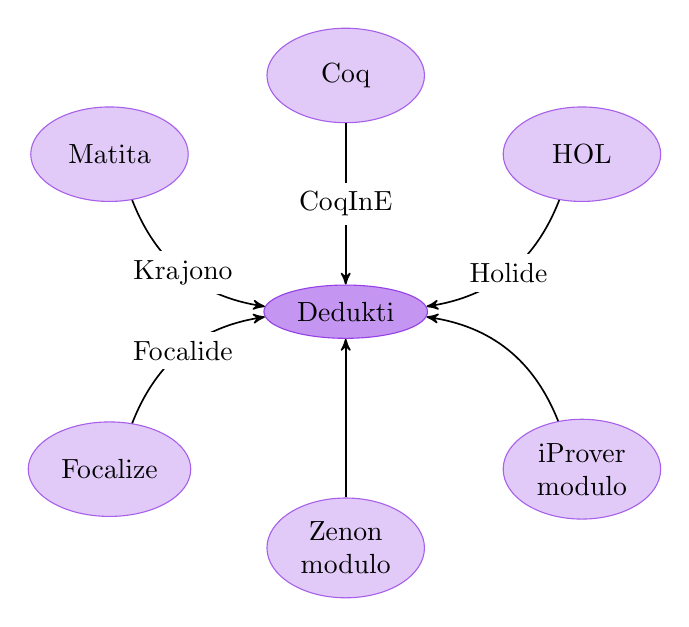
\begin{tikzpicture}
    [node distance=3cm,
    on grid,
    checker/.style = {shape=ellipse, draw=blue-violet!75, fill=blue-violet!25, align=center,
      minimum height=1.2cm, minimum width=2cm},
    dedukti node/.style = {shape=ellipse, draw=blue-violet!90, fill=blue-violet!50},
    post/.style={->, >=stealth', semithick}]

    \node [dedukti node] (Dedukti) {Dedukti};
    \node [checker] (Coq) [above=of Dedukti] {Coq}
    edge [post] node [fill=white,swap] {CoqInE} (Dedukti);
    \node [checker] (HOL) [right=of Coq, yshift=-1cm] {HOL}
    edge [post, bend left] node [fill=white,swap] {Holide} (Dedukti);
    \node [checker] (Matita) [left=of Coq, yshift=-1cm] {Matita}
    edge [post, bend right] node [fill=white,swap] {Krajono} (Dedukti);
    \node [checker] (Zenon modulo) [below=of Dedukti] {Zenon\\ modulo}
    edge [post] (Dedukti);
    \node [checker] (iProver modulo) [right=of Zenon modulo, yshift=1cm] {iProver\\modulo}
    edge [post, bend right]  (Dedukti);
    \node [checker] (Focalize) [left=of Zenon modulo, yshift=1cm] {Focalize}
    edge [post, bend left] node [fill=white,swap] {Focalide} (Dedukti);

    % \draw[very thick,dashed,->, blue] (Matita) .. controls ([yshift=-0.2cm]Dedukti) .. (HOL);
  \end{tikzpicture}
\end{center}
\end{document}